\newpage
\appendix


\section{Reproducible Audit}



To show the utility of Aequitas, we used it to audit ML models developed at the Center for Data Science and Public Policy, University of Chicago, being used to solve problems in different domains. However, we are not allowed to share the input data used in the audits. Here we present a short case study of one of our audits using a publicly available data set (COMPAS) from criminal justice. A Jupyter notebook containing the code to run this audit is available at the Aequitas Github repo \footnote{\url{https://bit.ly/2MP89VS}}.

The goal of COMPAS was to identify individuals who are at risk of recidivism to support pretrial release decisions. In a recent widely popularized investigation conducted by a team at ProPublica, Angwin et al. concluded that it was biased against black defendants. 

\subsection{Data}
The data is based on the Broward County data made publicly available by ProPublica \citep{angwin2016machine}. This data set contains COMPAS recidivism risk decile scores, 2-year recidivism
outcomes, and a number of demographic and variables on 7214 individuals who were scored
in 2013 and 2014. 

\subsection{Bias Audit using Aequitas}
We audited the predictions using Aequitas. We find that there is indeed unfairness (both unsupervised and supervised) in the model in all three attributes of interest: age, gender, and race. 

\begin{figure*}[h]
	\centering
	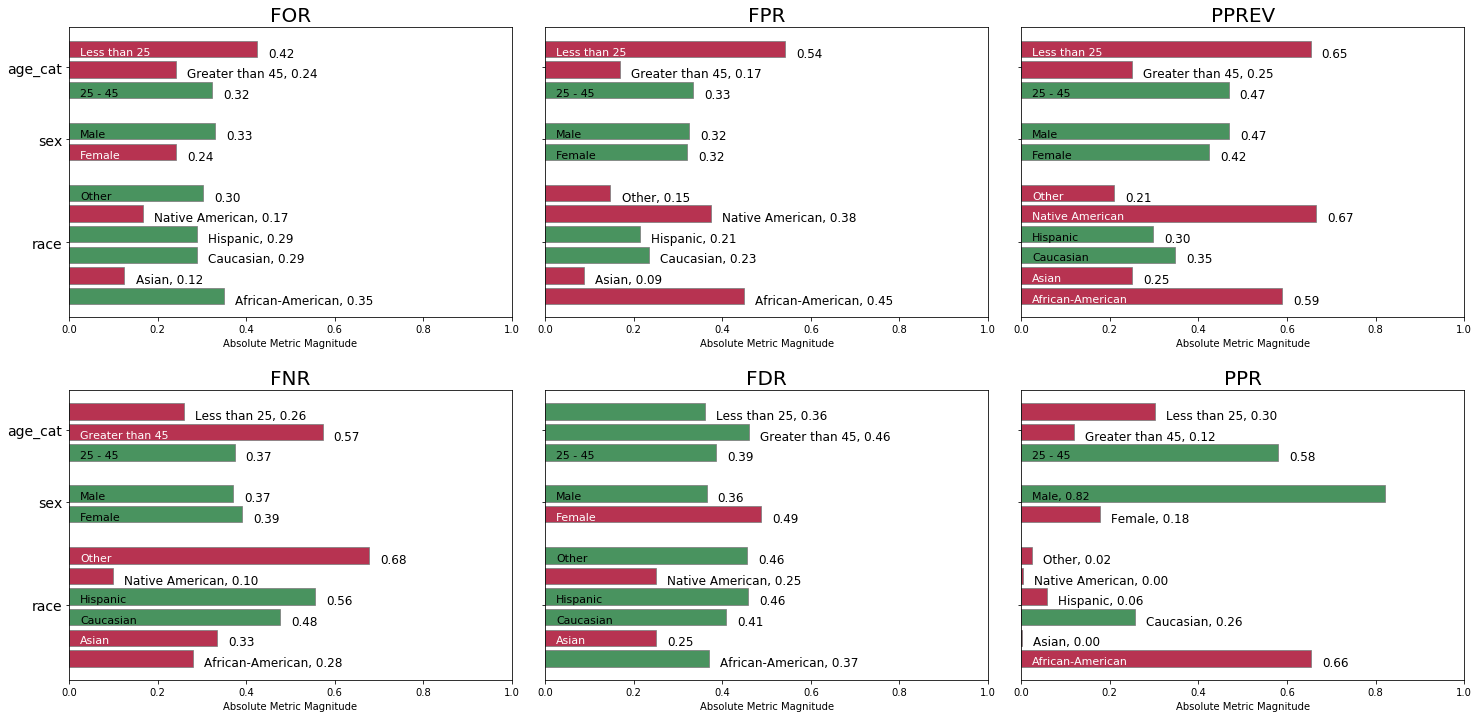
\includegraphics[width=1.0\linewidth]{fairness_group_all.png}
	\caption{Group metrics results for COMPAS. Bars in green/red represent groups that passed/failed the fairness test using $\uptau=0.8$. }
	\label{fig:group_metrics}
\end{figure*}

Figure \ref{fig:group_metrics} shows the detailed group metric results. Each row represents a specific attribute-value pair (gender:female), and each bar (column) represents a group metric of interest (False Positive Rate for example). Green bars represent groups for which the model does not exhibit bias within that metric. Red bars are those that are unfavorably biased compared to the reference group. In this case we used a fairness threshold $\uptau = 0.8$ and the results show that for every metric considered there is some kind of bias towards specific groups. For instance, PPR results show that COMPAS mostly consider as high risk people with age 18-25, Males and African-Americans and that compared to each group size, younger people, Native Americans and African-Americans are being selected disproportionally.


\begin{figure*}[h]
	\centering
	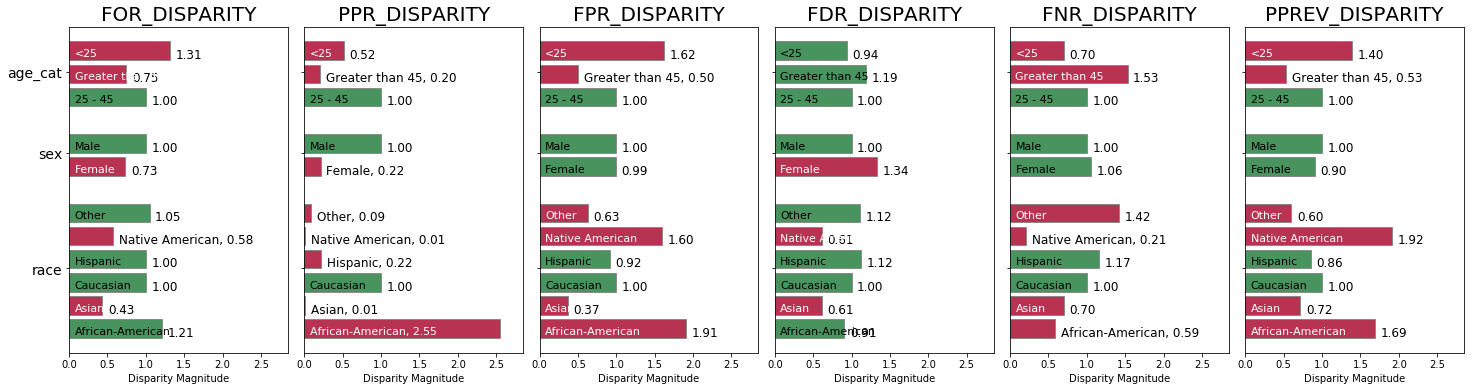
\includegraphics[width=1.0\linewidth]{fairness_disparity_all.png}
	\caption{Disparity metrics results for COMPAS. Bars in green/red represent groups that passed/failed the fairness test using $\uptau=0.8$. }
	\label{fig:disparity}
\end{figure*}

To easily visualize the disparities between the different groups, the tool also produces results for the bias measures. We then have to determine which bias measure is relevant for our setting. If the interventions we're focusing on in our setting are ``assistive'', we only need to consider Type II parity -- False Omission Rates (FOR) and False Negative Rates (FNR). This is because our interventions are preventative and designed to provide extra assistance to individuals. Providing this assistance to individuals who are false positives will not hurt them but missing individuals could be harmful to them.

If the interventions we're focusing on in our setting are ``punitive'', we  need to consider Type I parity -- False Discovery Rates (FDR) and False Positive Rates (FPR). This is because our interventions are punitive providing this intervention to individuals who are false positives will hurt them. Since in the COMPAS setting, the predictions are being used to make pretrial release decisions, we care about FPR and FDR Parity.

Looking at the figure \ref{fig:disparity} we can see that COMPAS is fair regarding the FDR for race but as ProPublica found, the FPR for African-Americans is almost twice as the FPR for Caucasians. For age we observe the same results for the same two metrics: FDR results are fair but FPR for <25 is 1.6X higher than 25-45. On the other hand, if we consider false positive errors distribution considering Sex we observe the contrary: the model is fair for FPR but the FDR of Female is 1.34 times higher than for Male. 

